\chapter{Metodología de investigación}
Para alcanzar el objetivo final es importante fijar unos pasos concretos a seguir. Por ello, en un primer lugar hemos estudiado el estado del arte, que nos permite conocer que herramientas se encuentran a nuestra disposición. A continuación tendremos que revisar el \textit{dataset} del que partimos, balanceándolo y añadiendo \textit{hard-negatives} que permitirán entrenar el modelo clasificador de forma que funcione correctamente en casos más difíciles. Tras haber preparado el dataset, entrenaremos el modelo clasificador sobre este.

En esta sección explicamos los conceptos más importantes que debemos entender si queremos comprender las decisiones que se han tomado y el funcionamiento de los modelos.

La implementación de los pasos que explicamos en este capítulo se encuentra en el repositorio de GitHub del proyecto \cite{repository}. La raíz del repositorio contiene los siguientes elementos:

\dirtree{%
    .1 /.
    .2 datasets/.
    .2 experiments/\DTcomment{implementación del TFG}.
    .2 papers/\DTcomment{algunas de las publicaciones utilizadas en su desarrollo}.
    .2 report/\DTcomment{memoria en formato \LaTeX}.
    .2 slides/.
    .2 README.md.
}

El código se utiliza para ejecutar los experimentos que se tratarán en el próximo capítulo.

\newpage
\section{Balanceo del dataset}
El dataset, entregado por los científicos de la Universidad de Negev, contiene ejemplos positivos y negativos. Todas las imágenes son diferentes, presentan elementos con distintos trazados de línea, tamaños, colores... Originalmente se encuentran en formato .png.

Los ejemplos positivos son imágenes de moléculas extraídas de publicaciones. La mayoría son moléculas completas, aunque algunas parecen recortes de estructuras más grandes. En total tenemos 162 imágenes de este tipo.

\begin{figure}[H]
\centering
    \fbox{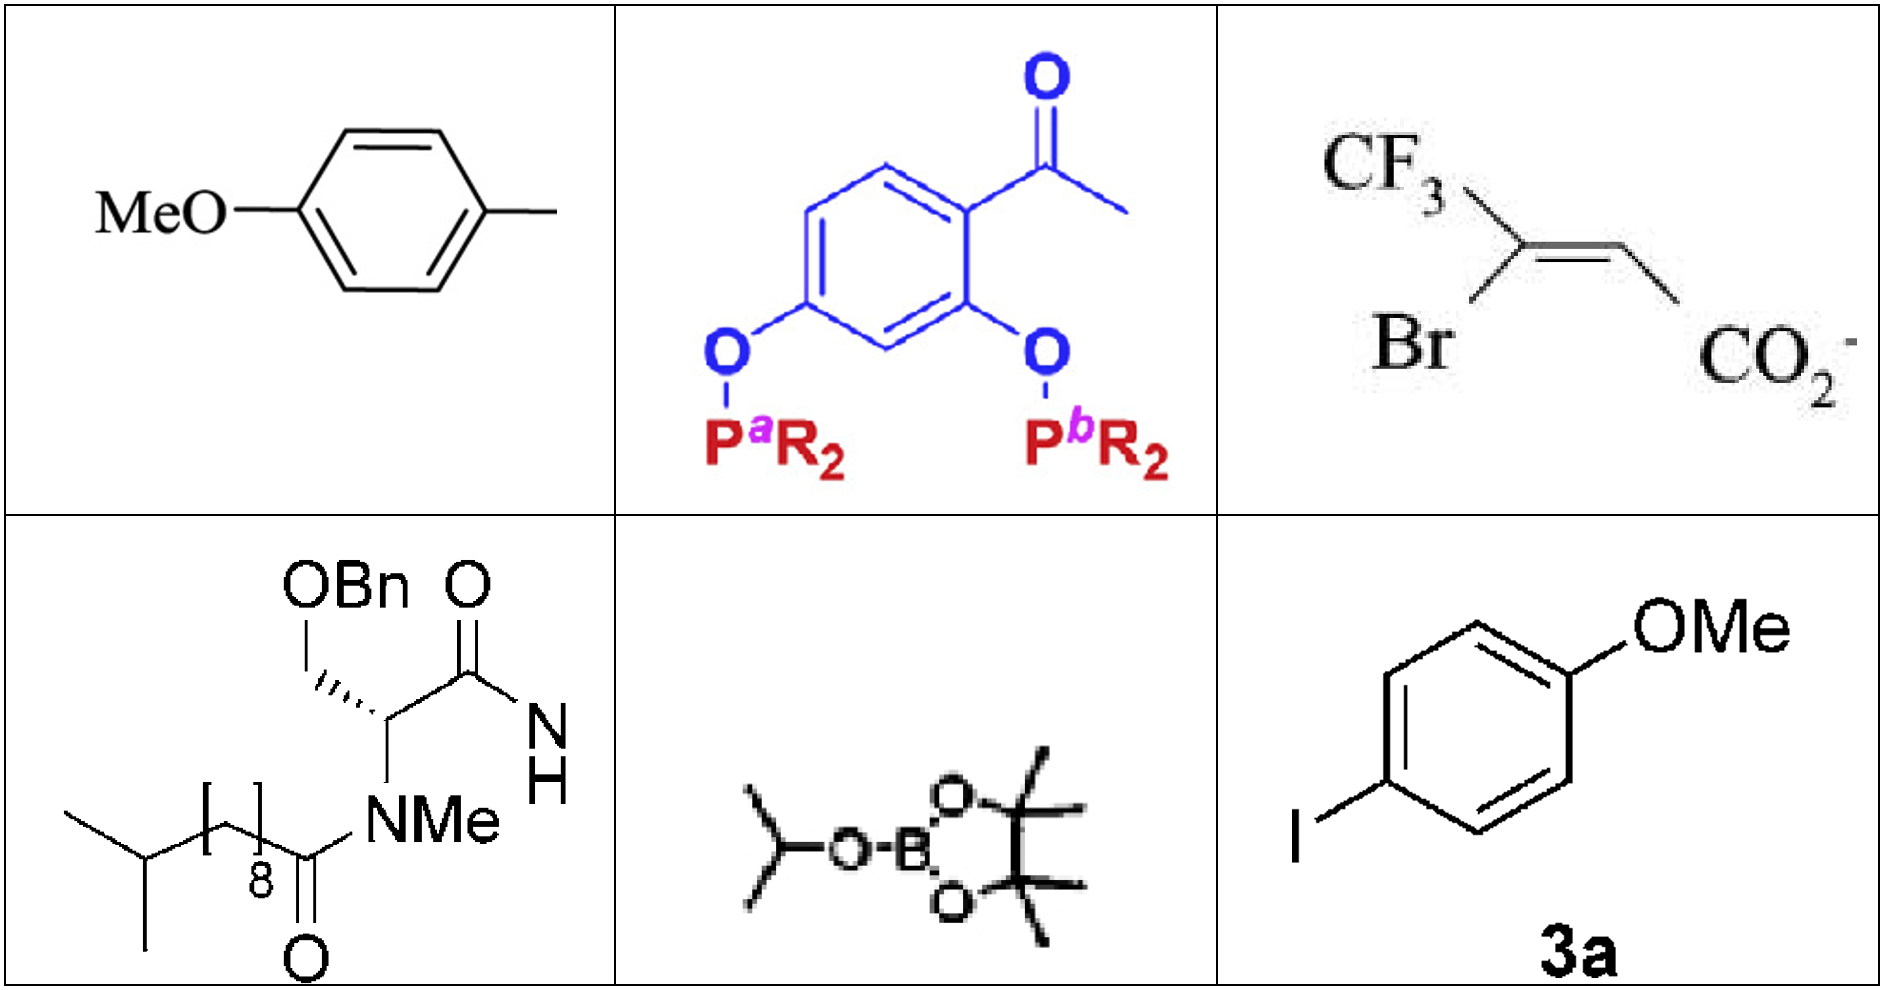
\includegraphics[scale=0.3]{imagenes/positive_examples.png}}  
    \caption{Ejemplos de muestras positivas del dataset} 
\end{figure}

Los ejemplos negativos son, en cambio, imágenes que contienen rectas, curvas y otras figuras que se parecen a las formas que adquiere una molécula, pero no lo son. La diversidad de estas imágenes es muy alta, como se puede observar en la figura \ref{fig:negative_examples}. En esta categoría hay más imágenes, 800 en total.

\begin{figure}[H]
\centering
    \fbox{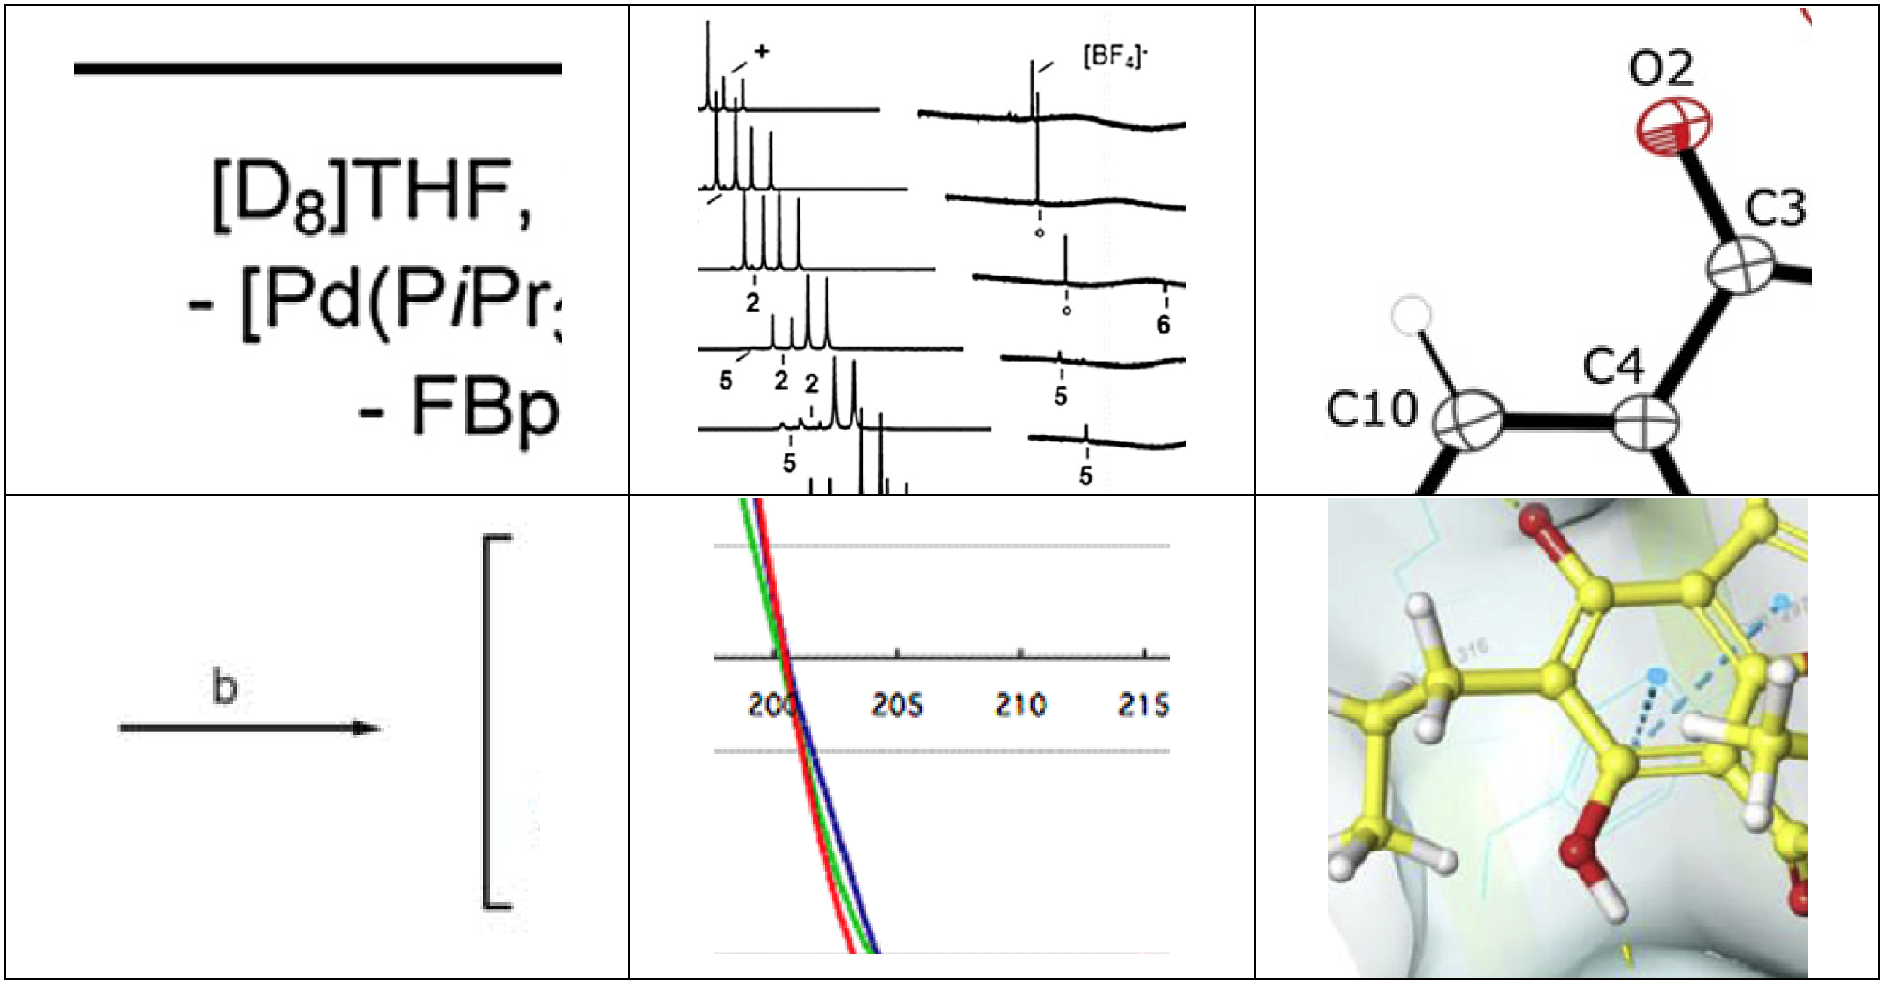
\includegraphics[scale=0.3]{imagenes/negative_examples.png}}  
    \caption{Ejemplos de muestras negativas del dataset}
    \label{fig:negative_examples}
\end{figure}

Estas imágenes necesitan un preprocesamiento, es necesario elegir el formato con el que se va a trabajar y dimensionarlas para que todas tengan el mismo tamaño. Debido a que el canal alfa del formato .png no se está aprovechando, decidimos convertirlas a formato .jpg y así trabajar con tres canales en nuestros modelos. Además, el modelo generativo que utilizamos está diseñado para trabajar con imágenes con este número de canales, así que será lo más adecuado.

Lo más conveniente sería dimensionar todas las imágenes al tamaño de la más grande, así no se perdería información. Pero esto puede suponer un problema, ya que existen algunas que superan los 700x700 píxeles, y cuanto mayor es su resolución más parámetros necesitan almacenar los modelos, dando lugar a altos tiempos de ejecución, y sobre todo, a problemas con la memoria de la GPU, problemas observables especialmente con el modelo generativo. Las GPUs del clúster no tienen capacidad para almacenar modelos con tantos parámetros, por lo que decidimos reducir el tamaño de las imágenes a 256x256. 

También mencionar el limitado número de ejemplos positivos que tenemos en comparación con negativos: estamos ante un conjunto de datos desbalanceado. En el momento de entrenar el clasificador, tendremos que conseguir que esté balanceado, ya sea reduciendo el número de ejemplos negativos utilizado o aplicando \textit{data augmentation} sobre los positivos. En este trabajo elegimos la segunda opción, ya que en Aprendizaje Automático cuantos más datos se utilizan en el entrenamiento, mejores modelos se obtienen. 

La técnica de \textit{data augmentation} consiste en aumentar el tamaño del conjunto de datos completándolo con imágenes alteradas de este. Existen bibliotecas en lenguajes de programación como Python que facilitan en gran medida esta tarea, ya que permiten indicar, entre una serie de transformaciones ya implementadas, cuáles queremos aplicar \cite{imgaug}. En nuestro caso vamos a crear tres \textit{data augmentation} diferentes, y comprobaremos cuál funciona mejor en los experimentos. La primera realizará transformaciones suaves, la segunda algo más fuertes y la tercera bastante disruptivas.

\begin{algorithm}[H]
    \caption{\textit{Data augmentation} 1: Transformaciones suaves}
\begin{algorithmic}[1]
    \State A\_veces(50\%, DesenfoqueGaussiano(sigma=[0, 0.5]))
    \State Escalar(x: [80\%, 100\%], y: [80\%, 100\%])
    \State Rotar([-25º, +25º])
    \State Estirar([-5,5])
\end{algorithmic}
\end{algorithm}

A cada imagen del conjunto de datos se le aplicarán estas cuatro transformaciones, la primera solamente con un 50\% de probabilidad. Los parámetros de cada transformación vienen dados en un rango, de forma que se elige un valor aleatorio en este.

% \begin{figure}[H]
% \centering
%     \begin{subfigure}{.35\textwidth}
%         \centering
%         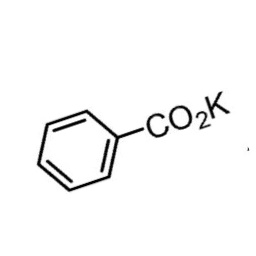
\includegraphics[width=1\linewidth]{imagenes/aug/180.jpg}
%     \end{subfigure}%
%     \begin{subfigure}{.35\textwidth}
%         \centering
%         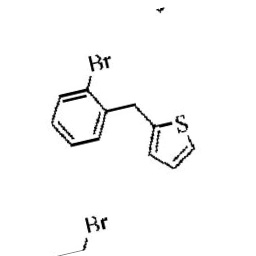
\includegraphics[width=1\linewidth]{imagenes/aug/193.jpg}
%     \end{subfigure}%

%     \bigskip

%     \begin{subfigure}{.35\textwidth}
%         \centering
%         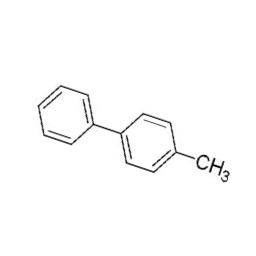
\includegraphics[width=1\linewidth]{imagenes/aug/224.jpg}
%     \end{subfigure}%
%     \begin{subfigure}{.35\textwidth}
%         \centering
%         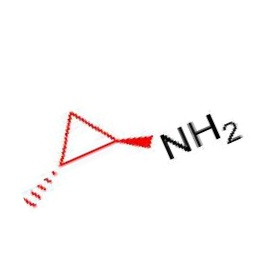
\includegraphics[width=1\linewidth]{imagenes/aug/370.jpg}
%     \end{subfigure}

%     \caption{Imágenes generadas aplicando \textit{data augmentation} 1}
% \end{figure}

% Algunos ejemplos son los que se muestran sobre este párrafo, se aprecian leves rotaciones y estiramientos de las imágenes, sin existir gran diferencia con las originales.

\begin{algorithm}[H]
    \caption{\textit{Data augmentation} 2: Transformaciones más fuertes}
\begin{algorithmic}[1]
    \State A\_veces(50\%, DesenfoqueGaussiano(sigma=[0, 0.5]))
    \State ContrasteLineal([0.75, 1.5])
    \State Escalar(x: [70\%, 100\%], y: [70\%, 100\%])
    \State Rotar([-45º, +45º])
    \State Estirar([-10,10])
    \State Trasladar(x: [-10\%, 10\%], y: [-10\%, 10\%])
    \State Multiplicar([0.8, 1.2], por\_canal=25\%)
    \State RuidoGaussianoAditivo(loc=0, escala=[0.0, 0.05*255])
    \State VoltearIzdaDcha(30\%)
\end{algorithmic}
\end{algorithm}

En este caso, utilizaremos transformaciones como Multiplicar (multiplica el valor de los píxeles de la imagen por un número entre 0.8 y 1.2), RuidoGaussianoAditivo (donde a cada píxel se le añade ruido generado mediante una distribución gaussiana centrada en 0 y con desviación entre 0 y 0.05*255) o VoltearIzqdaDcha, entre otras.

% \begin{figure}[H]
% \centering
%     \begin{subfigure}{.35\textwidth}
%         \centering
%         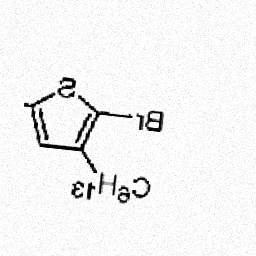
\includegraphics[width=1\linewidth]{imagenes/aug2/169.jpg}
%     \end{subfigure}%
%     \begin{subfigure}{.35\textwidth}
%         \centering
%         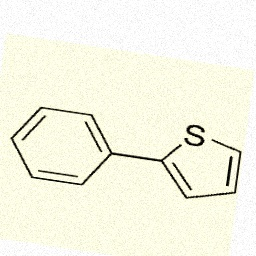
\includegraphics[width=1\linewidth]{imagenes/aug2/188.jpg}
%     \end{subfigure}%

%     \bigskip

%     \begin{subfigure}{.35\textwidth}
%         \centering
%         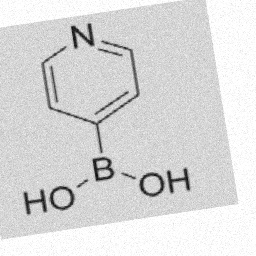
\includegraphics[width=1\linewidth]{imagenes/aug2/221.jpg}
%     \end{subfigure}%
%     \begin{subfigure}{.35\textwidth}
%         \centering
%         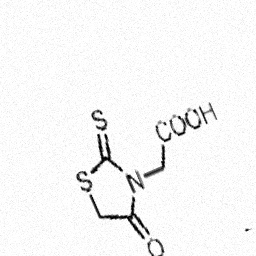
\includegraphics[width=1\linewidth]{imagenes/aug2/222.jpg}
%     \end{subfigure}

%     \caption{Imágenes generadas aplicando \textit{data augmentation} 2}
% \end{figure}

% En este caso se observan más cambios fundamentalmente debidos a las variaciones en contraste, al uso de ruido gaussiano y a la multiplicación, responsable de los cambios de color, ya que a veces se aplica a canales independientes. 

\begin{algorithm}[H]
    \caption{\textit{Data augmentation} 3: Transformaciones fuertes}
\begin{algorithmic}[1]
    \State A\_veces(50\%, DesenfoqueGaussiano(sigma=[0, 0.6]))
    \State ContrasteLineal([0.75, 2])
    \State Escalar(x: [70\%, 100\%], y: [70\%, 100\%])
    \State Rotar([-45º, +45º])
    \State Estirar([-10,10])
    \State Trasladar(x: [-20\%, 20\%], y: [-10\%, 10\%])
    \State Multiplicar([0.6, 1.4], por\_canal=25\%)
    \State RuidoGaussianoAditivo(loc=0, escala=[0.0, 0.05*255], por\_canal=30\%)
    \State VoltearIzdaDcha(20\%)
    \State VoldearArribaAbajo(20\%)
    \State A\_veces(70\%, TransformacionElastica(alfa=[0.75, 3], sigma=(0.2, 0.5)))
    \State UnoEntre(Nitidez(alfa=[0, 1], lightness=[0.5, 1.5]), Emboss(alfa=[0, 1], fuerza=[0.75, 2]))
    \State Dropout([0.01, 0.15], por\_canal=0.5)
\end{algorithmic}
\end{algorithm}
% TODO: Cómo se traduce emboss al español??

Finalmente, en esta versión de \textit{data augmentation} añadimos transformaciones que alteran en gran medida el aspecto de las imágenes. TransformacionElastica desplaza píxeles de una zona de la imagen a otra cercana, donde alfa controla la distancia con la que se produce el desplazamiento y sigma la suavidad de este, un valor bajo de sigma dará lugar a imágenes ruidosas y pixeladas. Nitidez aplica este efecto a la imagen y mezcla el resultado con la imagen original, la intensidad de la mezcla se controla con el parámetro alfa, mientras que el parámetro lightness controla el brillo de la imagen. Emboss da a la imagen un aspecto metálico, pronunciando las altas luces y sombras. Por último, Dropout da el valor 0 a cada pixel con una probabilidad entre 0.01 y 0.15. 

% \begin{figure}[H]
% \centering
%     \begin{subfigure}{.35\textwidth}
%         \centering
%         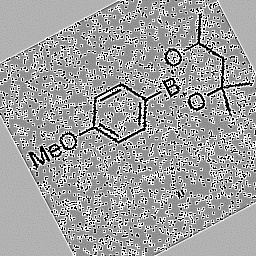
\includegraphics[width=1\linewidth]{imagenes/aug3/175.jpg}
%     \end{subfigure}%
%     \begin{subfigure}{.35\textwidth}
%         \centering
%         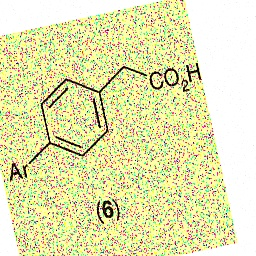
\includegraphics[width=1\linewidth]{imagenes/aug3/183.jpg}
%     \end{subfigure}%

%     \bigskip

%     \begin{subfigure}{.35\textwidth}
%         \centering
%         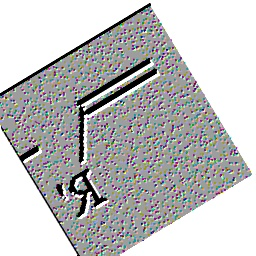
\includegraphics[width=1\linewidth]{imagenes/aug3/225.jpg}
%     \end{subfigure}%
%     \begin{subfigure}{.35\textwidth}
%         \centering
%         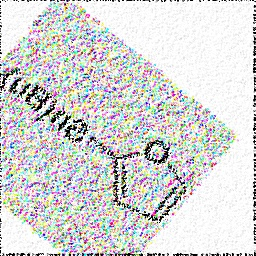
\includegraphics[width=1\linewidth]{imagenes/aug3/271.jpg}
%     \end{subfigure}

%     \caption{Imágenes generadas aplicando \textit{data augmentation} 3}
% \end{figure}

% En esta última versión las transformaciones son bastante agresivas. Se introduce mucho ruido en las imágenes y las rotaciones y los cambios en el contraste son fuertes.

El \textit{dataset} original y los derivados obtenidos al aplicar \textit{data augmentation} se almacenarán en el directorio \textit{datasets/} del repositorio, como se describe en el siguiente árbol:

\vspace{0.3cm}
\dirtree{%
    .1 datasets/.
    .2 negev/.
    .3 articles\_molecules/\DTcomment{ejemplos positivos}.
    .4 preprocess256/.
    .5 aug/\DTcomment{\textit{data augmentation} 1}. 
    .6 1.png.
    .6 2.png.
    .6 \ldots.
    .5 aug2/\DTcomment{\textit{data augmentation} 2}.
    .6 1.png.
    .6 2.png.
    .6 \ldots.
    .5 aug3/\DTcomment{\textit{data augmentation} 3}.
    .6 1.png.
    .6 2.png.
    .6 \ldots.
    .5 1.png.
    .5 2.png.
    .5 \ldots.
    .4 1.png.
    .4 2.png.
    .4 \ldots.
    .3 not\_molecules/\DTcomment{ejemplos negativos}.
}

\newpage
Como resumen, el siguiente gráfico recoge los diferentes conjuntos de datos que obtendremos tras este proceso de data augmentation:
\begin{figure}[H]
    \centering
        \fbox{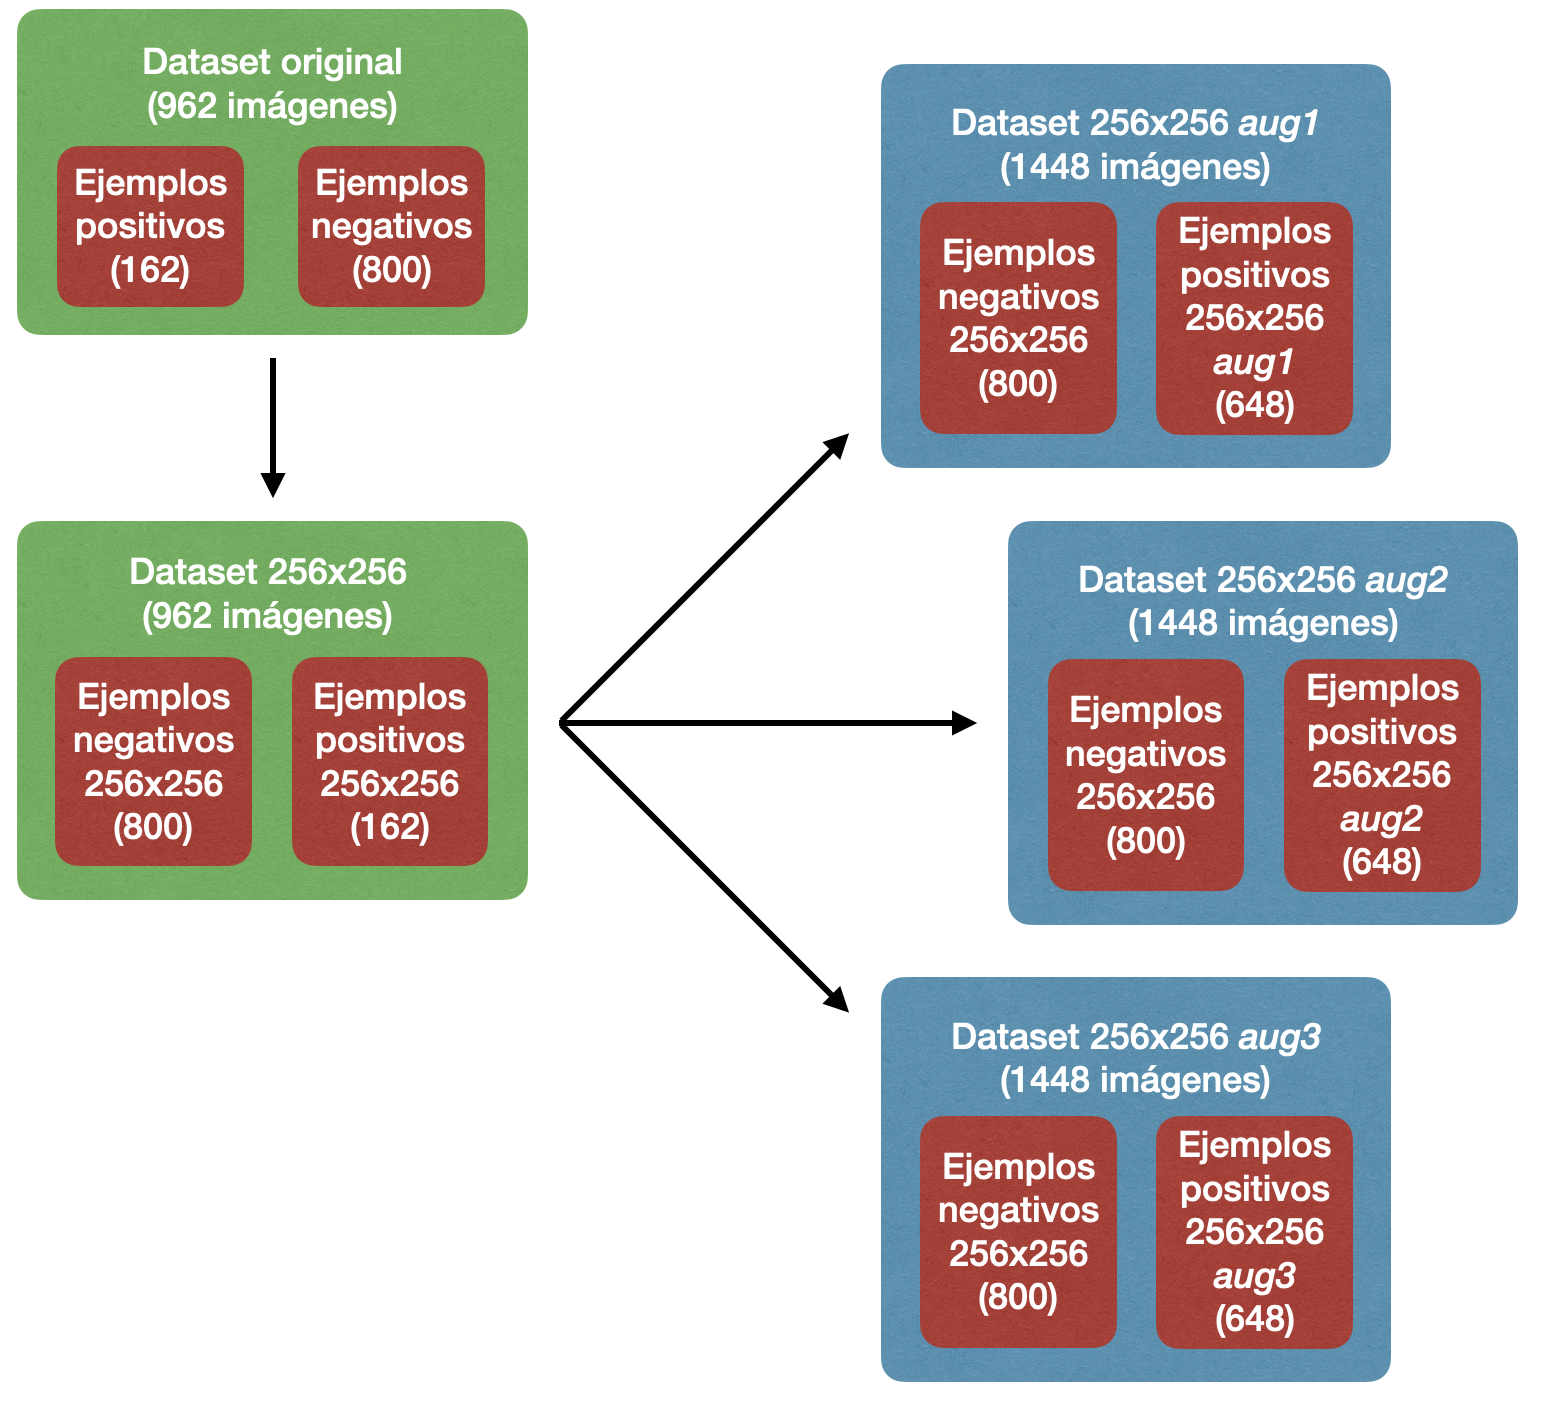
\includegraphics[scale=0.42]{imagenes/metodologia/datasets.png}}  
        \caption{Diferentes \textit{datasets} generados a partir del original} 
    \end{figure}

Las secuencias \textit{data augmentation} se aplicarán en tres ocasiones sobre el conjunto de ejemplos positivos, por lo que cuadruplican su tamaño inicial: 162 + 3*162 = 648

Ahora ya tenemos un \textit{dataset} razonablemente balanceado (800 ejemplos negativos vs 648 positivos), bueno, en concreto tres \textit{datasets}. Tras realizar las pruebas experimentales decidiremos cuál es el más adecuado, de forma que las imágenes generadas mediante \textit{data augmentation} aporten una diversidad razonable al conjunto pero sin excederse, para posteriormente utilizarlo para entrenar el clasificador.



\newpage
\section{Generación de \textit{hard negatives}}
Tras balancear los dataset con \textit{data augmentation}, procedemos a generar \textit{hard negatives}. Este tipo de ejemplos negativos son aquellos que se encuentran en el límite de lo que es negativo y positivo, aquellos que a los modelos de Aprendizaje Automático les cuesta clasificar. Incorporar este tipo de imágenes al conjunto de entrenamiento permite que el modelo sea más preciso en casos extremos y por tanto que funcione mejor.

\begin{figure}[H]
\centering
    \fbox{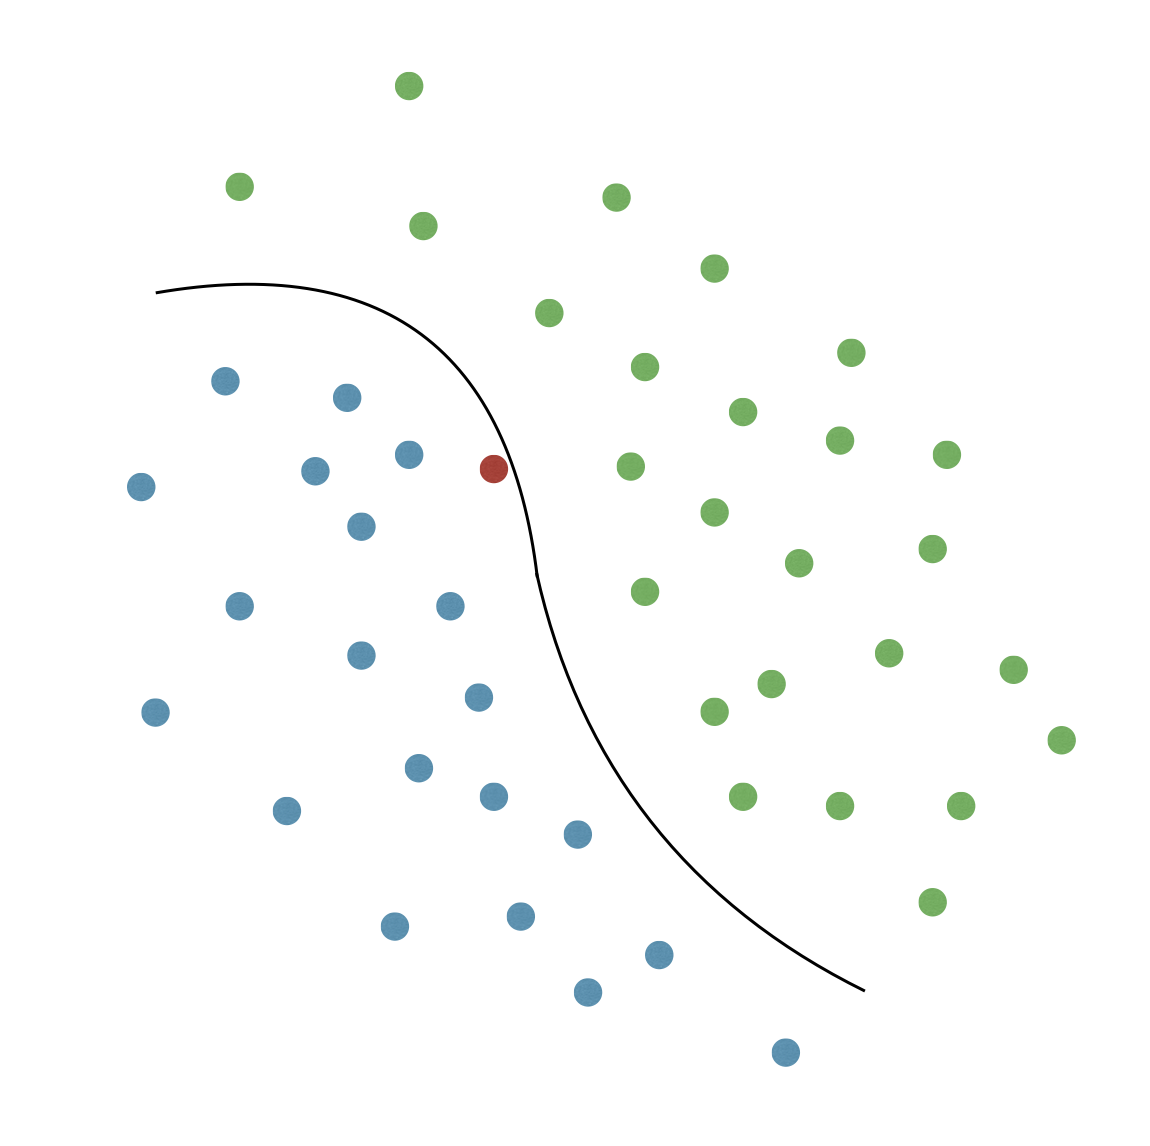
\includegraphics[scale=0.36]{imagenes/metodologia/hard_negatives.png}}  
    \caption{Límite de decisión separando dos clases. El individuo en rojo representa un \textit{hard negative} perteneciente a la clase azul, ya que se encuentra muy cercano al límite de decisión.} 
\end{figure}

% Una vez generados los \textit{hard negatives}, prepararemos dos datasets finales para entrenar el clasificador se añadirán al conjunto de datos final con el que entrenaremos el clasificador. Realmente no se añadirán, sino que sustituirán algunos de los ejemplos negativos originales, ya que sino volveríamos a encontrarnos frente a un \textit{dataset} no balanceado. Entrenaremos el clasificador de dos formas

La generación de estos ejemplos la vamos a realizar utilizando el modelo desarrollado por Esser et al. \cite{esser2021taming}, descrito en la revisión del estado del arte de este TFG. Para ello, entrenaremos el modelo sobre los ejemplos positivos del conjunto de datos de forma que sea capaz de generar imágenes que recuerden a moléculas sin que sean demasiado realistas. 

Se entrenará el modelo sobre los tres conjuntos de datos aumentados, aunque también se realizarán pruebas sobre el \textit{dataset} original. El entrenamiento se realizará durante diferentes épocas, y se comprobará visualmente cuál es el número adecuado. En concreto, sobre cada conjunto de datos, se prevé probar con 70, 90, 110, 130, 150 y 170 épocas. Si fuera necesario realizar más experimentos con diferentes valores, se realizarían también. Discutiremos esto más a fondo en el capítulo siguiente.

\begin{figure}[H]
\centering
    \fbox{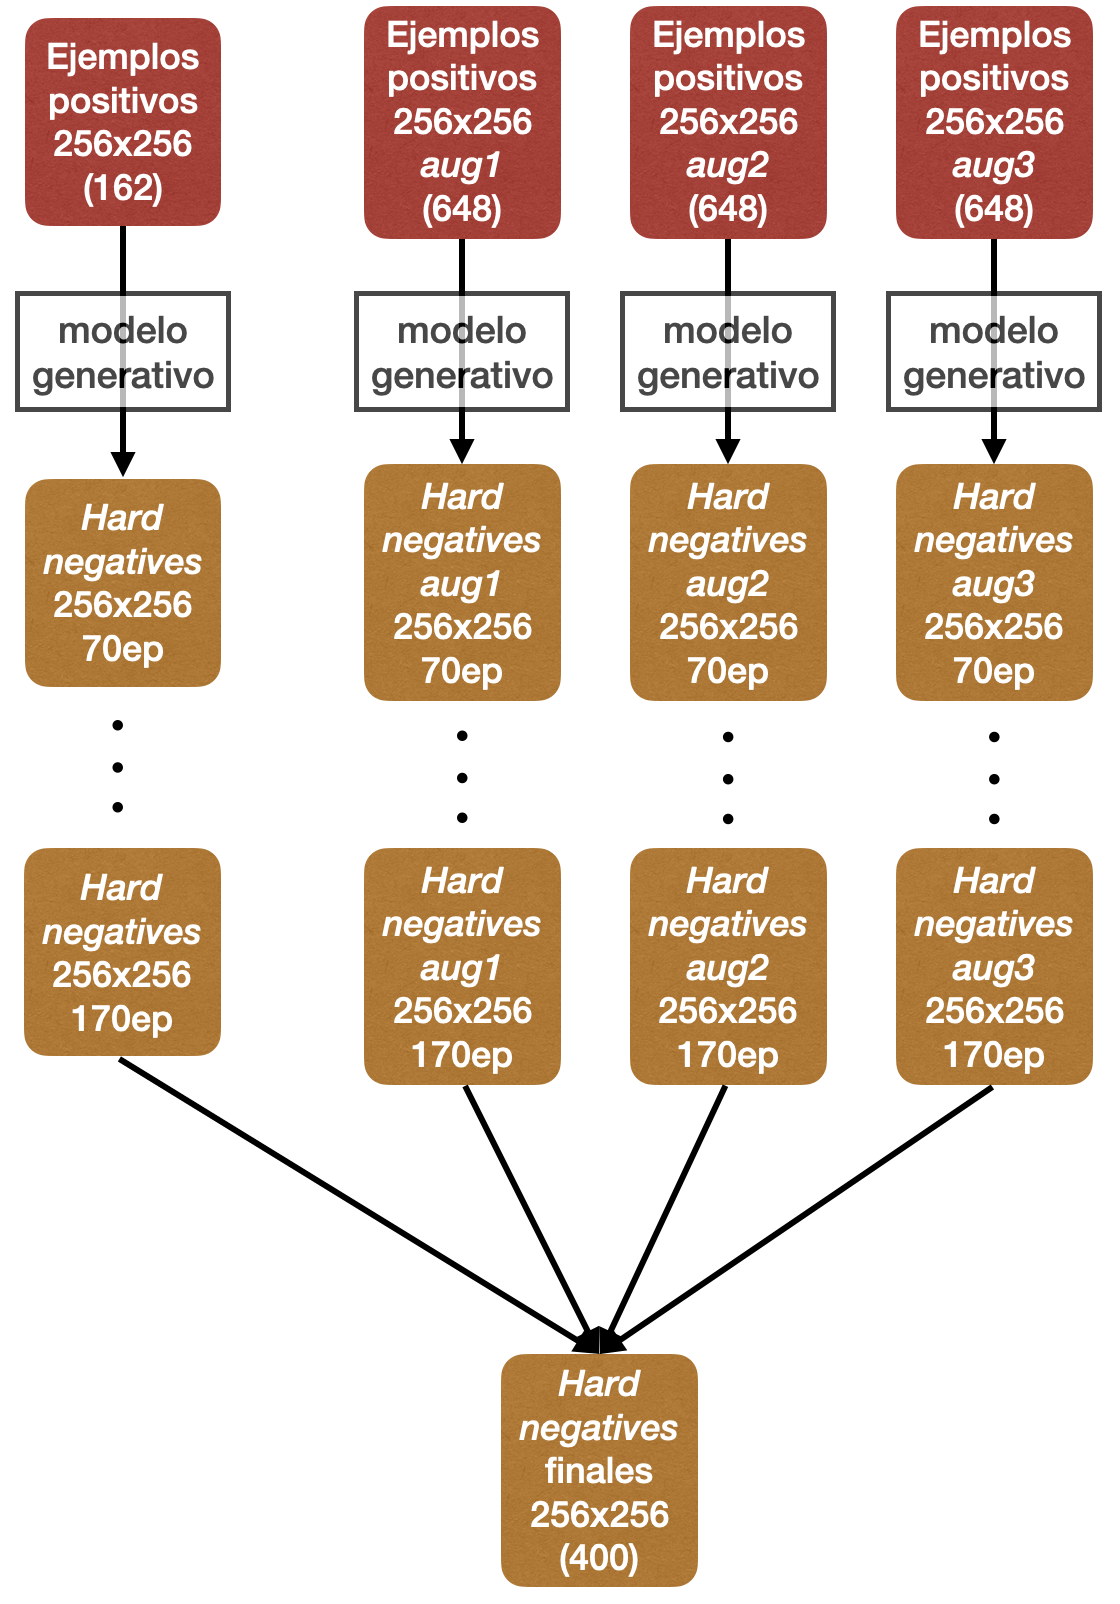
\includegraphics[scale=0.42]{imagenes/metodologia/generate_hard_negatives.png}}  
    \caption{Diferentes \textit{hard negatives} obtenidos entrenando el modelo con diferentes \textit{data augmentation} y número de épocas.} 
\end{figure}
    
Tras realizar los experimentos, se escogerá el modelo (o los modelos) que generen \textit{hard negatives} de mayor calidad. Esta elección se realizará de forma visual. Con los modelos elegidos se creará un conjunto de \textit{hard negatives} finales.



% que sustituirán a una parte de los ejemplos negativos que ya teníamos en el \textit{dataset} original, concretamente 400 ejemplos.




El directorio que recoge la implementación de todo este proceso es el siguiente:

\vspace{0.3cm}
\dirtree{%
    .1 /experiments/.
    .2 taming\_transformers/.
    .3 taming-transformers/.
    .3 data\_generation\_and\_augmentation.ipynb.
    .3 sampling\_experiment.ipynb.
    .3 sample\_and\_clean\_molecules.ipynb.
    .3 functions.py.
}

El subdirectorio \textit{taming\_transformers} contiene la implementación del modelo generativo proporcionada por sus autores \cite{taming-transformers-github}. 

\textit{{data\_generation\_and\_augmentation.ipynb}} contiene el código que preprocesa las imágenes, transformándolas de forma que tengan el mismo tamaño, y que aplica las tres secuencias de \textit{data augmentation} que hemos comentado.

\textit{sampling\_experiment.ipynb} es un cuaderno que, una vez entrenados los modelos, permite cargarlos y generar imágenes sintéticas a partir de otra imagen de entrada. Se utiliza para comprobar a partir de que \textit{dataset} se generan mejores resultados y con qué número de épocas. Es importante saber que este modelo generativo necesita de una imagen condicionante para generar una imagen sintética: probaremos con distintos tipos, entre ellas ruido, para comprobar con cuáles se obtienen mejores resultados.

\textit{sample\_and\_clean\_molecules.ipynb} nos permite generar un lote de imágenes sintéticas indicando el modelo que queremos utilizar y las propiedades del ruido, en concreto de ruido perlín, ruido que explicaremos en los experimentos. También creará el \textit{dataset} final que contiene \textit{hard negatives}.


% conjunto de datos sin aplicarles \textit{data augmentation} y haremos lo mismo aplicando \textit{data augmentation} 1, \textit{data augmentation} 2 y \textit{data augmentation} 3. En estos tres últimos casos, el número de imágenes utilizado para entrenar se multiplica por 4, ya que aplicamos las secuencias de transformaciones 3 veces. 

\newpage
\section{Clasificación de imágenes}
El segundo objetivo de este proyecto consiste en construir un clasificador capaz de separar las imágenes que contienen estructuras de moléculas de aquellas que no. Hasta ahora hemos preparado el \textit{dataset} con el que se va a entrenar este modelo y hemos generado \textit{hard negatives} que pueden ayudar a crear un clasificador más robusto.

En concreto vamos a trabajar con dos \textit{datasets}, no solo con uno: el que ha sido balanceado pero no contiene \textit{hard negatives} y el que sí los contiene. Entregaremos a los científicos de la Universidad de Negev ambos clasificadores. Para implementarlos utilizamos la biblioteca Pytorch ya expuesta en el capítulo estado del arte.

A priori no podemos conocer que arquitectura funcionará mejor para este problema, por lo que implementaremos varias y compararemos su rendimiento. Vamos a elegir una de tamaño pequeño, otra de tamaño mediano y otra de tamaño grande y comparar cuál es la más adecuada:
\begin{itemize}
    \item \textbf{LeNet5:} Modelo propuesto por Yann LeCun en 1998 \cite{lecun1998gradient}, fue una de las primeras redes convolutivas de la historia. Se diseñó con el propósito de reconocer imágenes de dígitos numéricos, y tras compararse su rendimiento con otros modelos en uso, se demostró que los sobrepasaba. Esto atrajo a muchos investigadores a esta incipiente línea de investigación y sentó las bases para las arquitecturas del futuro.
    \item \textbf{AlexNet:} Propuesto por Alex Krizhevsky en 2012 \cite{krizhevsky2012imagenet}, consiguió mejorar por un alto porcentaje a la siguiente mejor solución en el concurso ImageNet Large Scale Visual Recognition Challenge. La ventaja de este modelo frente a otros fue su profundidad, que le permitía reconocer imágenes más complejas con mayor precisión. Esto conllevó un aumento del número de parámetros y del tiempo de entrenamiento, que fue contrarrestado por el uso de GPUs que permitieron la paralelización. Para combatir el sobreajuste se utilizó \textit{dropout}, donde los enlaces entre neuronas se desconectaban con una determinada probabilidad durante cada iteración del entrenamiento.
    \item \textbf{VGG16:} Desarrollado por el Visual Geometry Group (de sus siglas procede el nombre del modelo) de la Universidad de Oxford \cite{https://doi.org/10.48550/arxiv.1409.1556}, fue el ganador del concurso ImageNet en su edición de 2014. Una de las características que le permitió mejorar frente a otros modelos fue el uso de \textit{kernels} convolutivos de pequeño tamaño (3x3). Se presentaron varias versiones del algoritmo, cada una con un número de capas diferente. La que nosotros utilizamos, VGG16, cuenta con 16 capas.
\end{itemize}

En un principio, cada uno de estos modelos se diseñó para trabajar con un tamaño de imágenes y de salida específicos, pero nosotros los adaptamos para funcionar sobre imágenes 256x256 y vectores \textit{one-hot}. Estos vectores se utilizan en problemas de clasificación, de forma que cada coordenada del vector representa una de las clases (en nuestro caso dos clases, imagen de molécula o no). Cada coordenada se conoce como \textit{logit}.

Tras la implementación con estos cambios, el número de parámetros se incrementa. Por ejemplo, LeNet5 contaba originalmente con 62006 parámetros al trabajar con imágenes 28x28 y un vector de salida de tamaño 10, pero tras los cambios cuenta con 7393806. Las versiones modificadas de AlexNet y VGG16 cuentan respectivamente con 58289538 y 153263298 parámetros.

Cada uno de estos modelos tiene diferentes hiperparámetros configurables: el tamaño del lote de entrenamiento (\textit{batch size}), el optimizador que modifica los parámetros en cada iteración, la inicialización de los pesos, etc. Determinados valores en estos hiperparámetros hacen que los modelos produzcan peores o mejores resultados, por lo que es importante elegir valores adecuados. Es imposible probar todos los valores posibles, por lo que seleccionamos algunos que creemos que pueden dar buenos resultados y realizamos una comparativa: esto es lo que se conoce como \textit{grid search}.

Vamos a trabajar con tres hiperparámetros. Aunque podríamos hacer pruebas con más, el número de modelos a entrenar crecería exponencialmente:
\begin{itemize}
    \item \textbf{Tasa de aprendizaje (\textit{Learning rate}):} Es probablemente el hiperparámetro más importante. Si le damos un valor demasiado bajo, los pesos del modelo variarán en muy poca medida en cada iteración y el error decrecerá muy lentamente. Si su valor es muy alto, es posible que el valor de los pesos y del error oscile y el algoritmo no converja. Es conveniente probar con diferentes posibilidades: en nuestro caso vamos a comprobar el rendimiento de los modelos tomando 0.5, 0.05, 0.005, 0.0005 y 0.00005 como posibles valores. \cite{berzal2018redes}
    \item \textbf{Inicialización de los pesos:} Las redes neuronales dependen en gran medida de la inicialización de los pesos. Si todas las neuronas se inicializasen con el mismo valor, el modelo no sería capaz de aprender nada, ya que la derivada del gradiente sería la misma para todas. Las que vamos a utilizar son: \cite{pytorch-doc}
    \begin{itemize}
        \item \textit{He:} utilizada por defecto en PyTorch en sus capas completamente conectadas y convolutivas, He (también conocida como Kaiming) genera valores aleatorios a partir de una distribución uniforme $\mathcal{U}(-bound, bound)$, donde $bound = gain * \sqrt{\frac{3}{fan\_in}}$. El parámetro $fan\_in$ depende de la entrada a la neurona. Por otro lado, en la inicialización por defecto de PyTorch $gain$ depende de $a = \sqrt{5}$.
        \item \textit{Xavier:} Los valores aleatorios son generados a partir de una distribución uniforme $\mathcal{U}(-a, a)$, donde $a = \sqrt{\frac{6}{fan\_in + fan\_out}}$. 
    \end{itemize}
    Una correcta inicialización de los pesos evita el problema de la evanescencia del gradiente (durante el entrenamiento, este se vuelve cada vez menor aproximándose a cero, de forma que los pesos no cambian) y el de la explosión del gradiente (este toma valores cada vez mayores, de forma que los pesos cambian en gran medida y el algoritmo diverge).
    \item \textbf{Algoritmo de optimización:} Como muchos otros algoritmos de aprendizaje automático, los de aprendizaje profundo son problemas de optimización donde se intenta reducir el error de una función objetivo $f$ definida sobre un conjunto de datos de entrenamiento. En muchas ocasiones, este proceso de optimización se realiza de forma numérica, una forma de hacerlo es a partir del cálculo del gradiente descendiente, un proceso costoso por tener que calcular en numerosas ocasiones el valor de la función $f$ y de su derivada. La elección del algoritmo de optimización es importante, ya que de él dependen la convergencia a una buena solución y el actualizar los pesos de forma eficiente: \cite{berzal2018redes}
    \begin{itemize}
        \item \textit{SGD:} En el entrenamiento de redes neuronales, el gradiente se calcula a partir de los datos de entrenamiento. Si estos datos no son un conjunto representativo de la distribución real porque contienen ruido, la estimación no será correcta. El gradiente se puede calcular a partir de todos los datos de entrenamiento (aprendizaje por lotes), a partir de un subconjunto (aprendizaje por minilotes) o a partir de una única muestra (aprendizaje online). Cuantos más datos utilicemos para calcular el gradiente, menor será el error cometido al estimarlo, pero como hemos mencionado, los datos siempre pueden contener ruido y por tanto no podemos asegurar que los resultados sean correctos. El gradiente descendiente estocástico (\textit{Stochastic Gradient Descent}, SGD) engloba el aprendizaje por minilotes y el online, y aunque pueda parecer lo contrario por utilizar menos muestras en el cómputo del gradiente, mejora los resultados al permitir al algoritmo escapar de puntos de silla. Además, es mucho más eficiente ya que solo tiene en cuenta un número limitado de datos en el cómputo.
        \item \textit{AdaDelta:} Es una extensión de AdaGrad (\textit{Adaptative Gradients}), un optimizador que dota a cada parámetro de una tasa de aprendizaje independiente y que va actualizando su valor durante la ejecución del algoritmo. AdaDelta resuelve el principal problema de Adagrad, la disminución prematura de las tasas de aprendizaje. Esto se debe a que Adagrad las calcula a partir del gradiente acumulado de todas las iteraciones, en cambio AdaDelta sólo utiliza las $n$ iteraciones anteriores.
        \item \textit{Adam:} Se podría considerar una extensión de AdaDelta en la que se utilizan momentos. En concreto, este algoritmo calcula la estimación del primer momento del gradiente (media) y del segundo momento (varianza). A partir de ellos se define la fórmula que da nombre a este algoritmo.
    \end{itemize}
\end{itemize}

En las ejecuciones que vamos a realizar, la función de coste que utilizamos es la función de entropía cruzada (\textit{Cross Entropy Loss}). Esta función integra la función de activación \textit{Softmax}, de forma que cada logit es transformado en un valor probabilístico entre 0 y 1. 

El algoritmo de aprendizaje intentará minimizar el valor de la función de entropía cruzada, es decir, tratará de minimizar la distancia entre las probabilidades devueltas por el modelo y la probabilidad real. Tras el entrenamiento, cuando realicemos una predicción, la clase a la que pertenecerá la muestra será aquella que esté representada por el \textit{logit} con mayor probabilidad. \cite{crossentropyloss}

\begin{figure}[H]
\centering
    \fbox{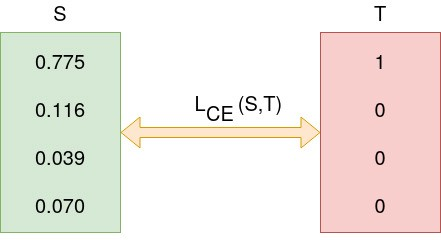
\includegraphics[scale=0.55]{imagenes/image_classification/crossentropyloss.jpeg}}
    \caption{La función de entropía cruzada $L_{CE}$ mide la distancia entre la probabilidad representada en el \textit{logit} $S$ y la probabilidad real representada mediante $T$ \cite{crossentropyloss}. Durante el entrenamiento, el algoritmo tratará de minimizar esta distancia.}
\end{figure}

\newpage
El objetivo es realizar la \textit{grid search} sobre los dos datasets que hemos comentado, de esta forma compararemos el rendimiento de los modelos según los hiperparámetros utilizados y nos quedaremos con aquellos que dan mejores resultados. Estos serán los que entreguemos a los científicos.

\begin{figure}[H]
\centering
    \fbox{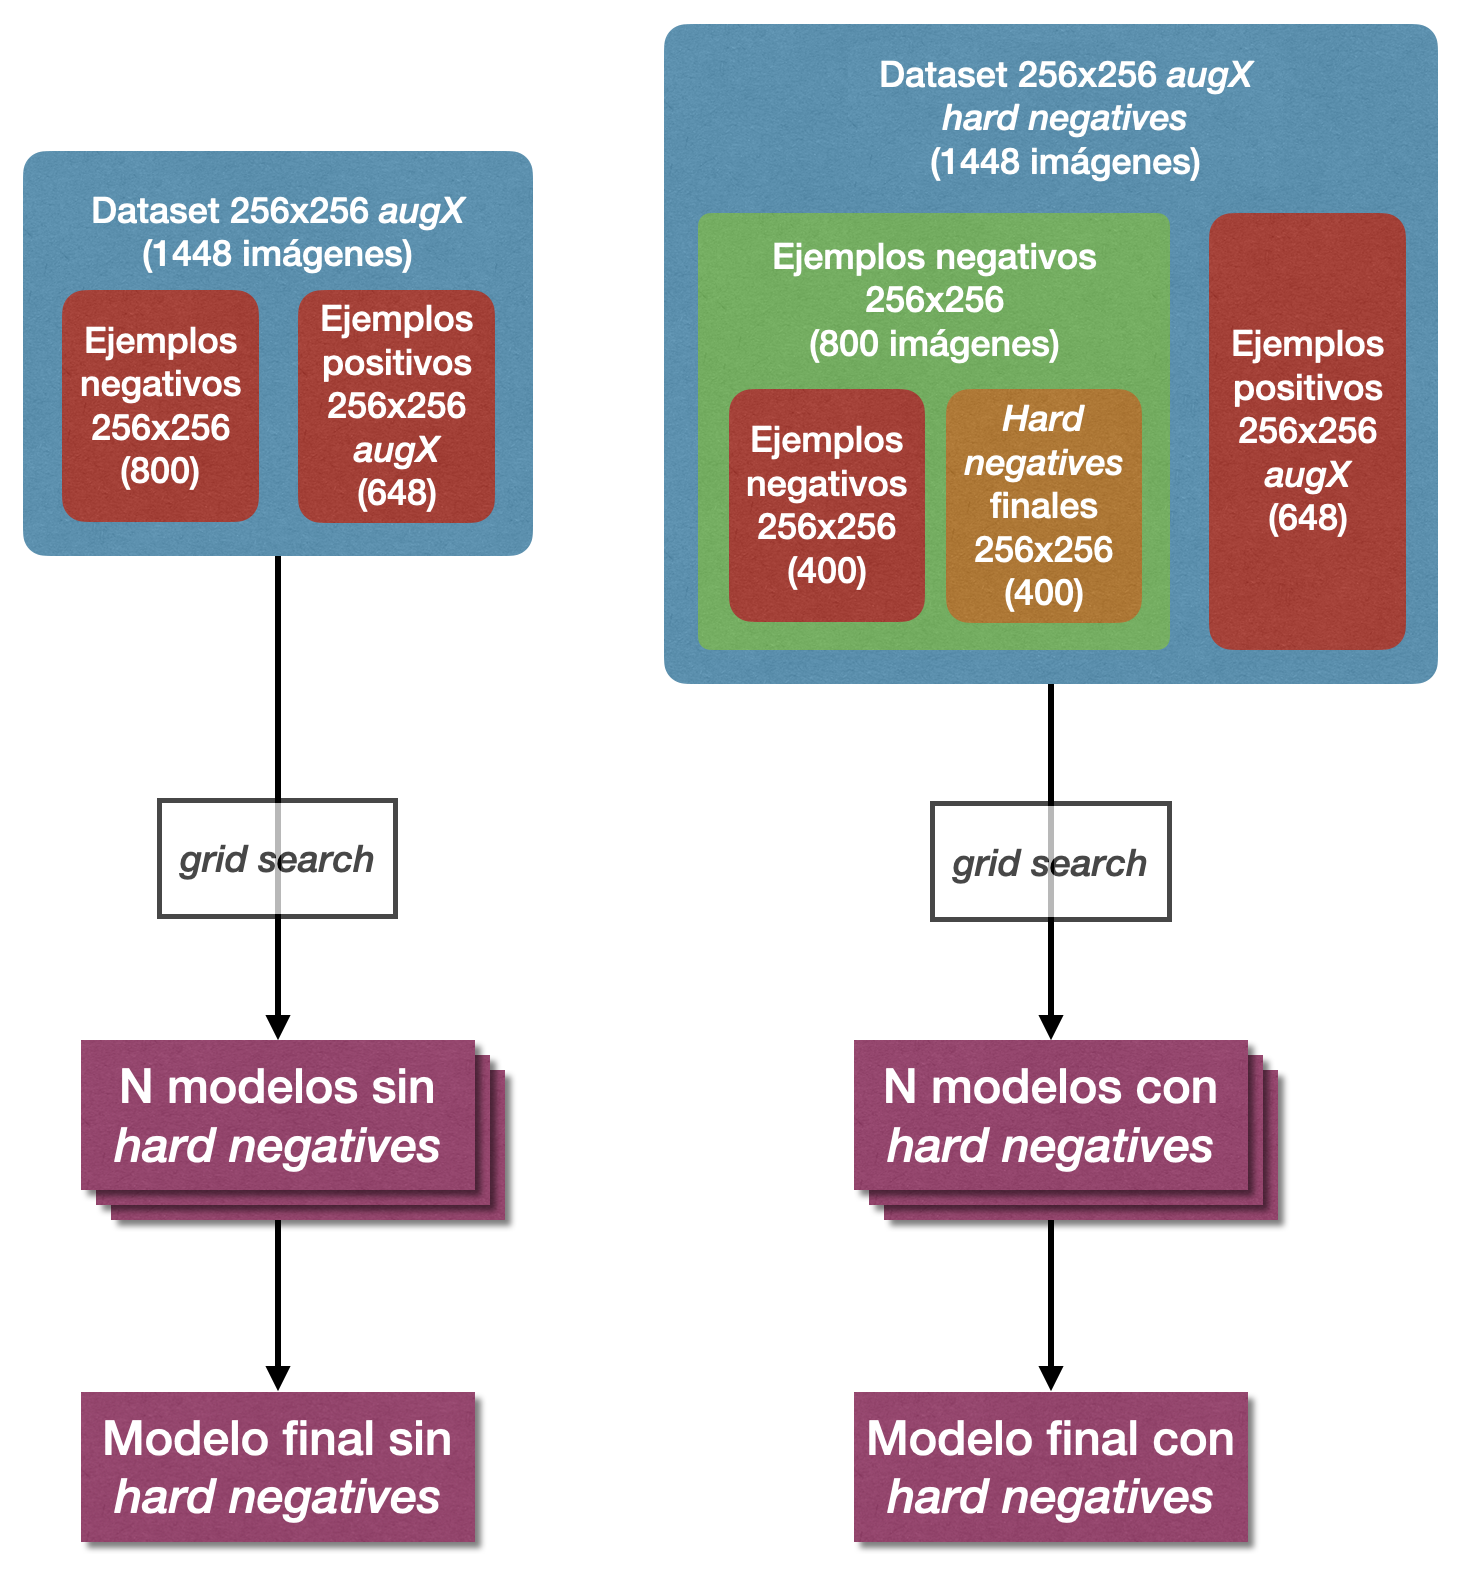
\includegraphics[scale=0.43]{imagenes/metodologia/grid_search.png}}  
    \caption{Realizamos una \textit{grid search} sobre ambos datasets, y elegimos el modelo que mejor resultado da sobre cada uno de ellos.} 
\end{figure}
















% Toda la implementación se encuentra en el repositorio de GitHub del proyecto \cite{repository}. La raíz del repositorio contiene los siguientes elementos:

% \dirtree{%
%     .1 /.
%     .2 datasets/.
%     .2 experiments/\DTcomment{implementación del TFG}.
%     .2 papers/\DTcomment{algunas de las publicaciones utilizadas en su desarrollo}.
%     .2 report/\DTcomment{memoria en formato \LaTeX}.
%     .2 slides/.
%     .2 README.md.
% }

% En el repositorio, el directorio datasets se encuentra vacío para no crear problemas con el sistema de control de versiones. En el README.md se indica un enlace donde se pueden descargar los datos que se deben colocar en el directorio.

% \newpage
% \section{Dataset utilizado}
% El dataset contiene ejemplos positivos y negativos. Todas las imágenes son diferentes, presentan elementos con distintos trazados de línea, tamaños, colores... Originalmente se encuentran en formato .png.

% Los ejemplos positivos son imágenes de moléculas extraídas de publicaciones. La mayoría son moléculas completas, aunque algunas parecen recortes de estructuras más grandes. En total tenemos 162 imágenes de este tipo.

% \begin{figure}[H]
% \centering
%     \fbox{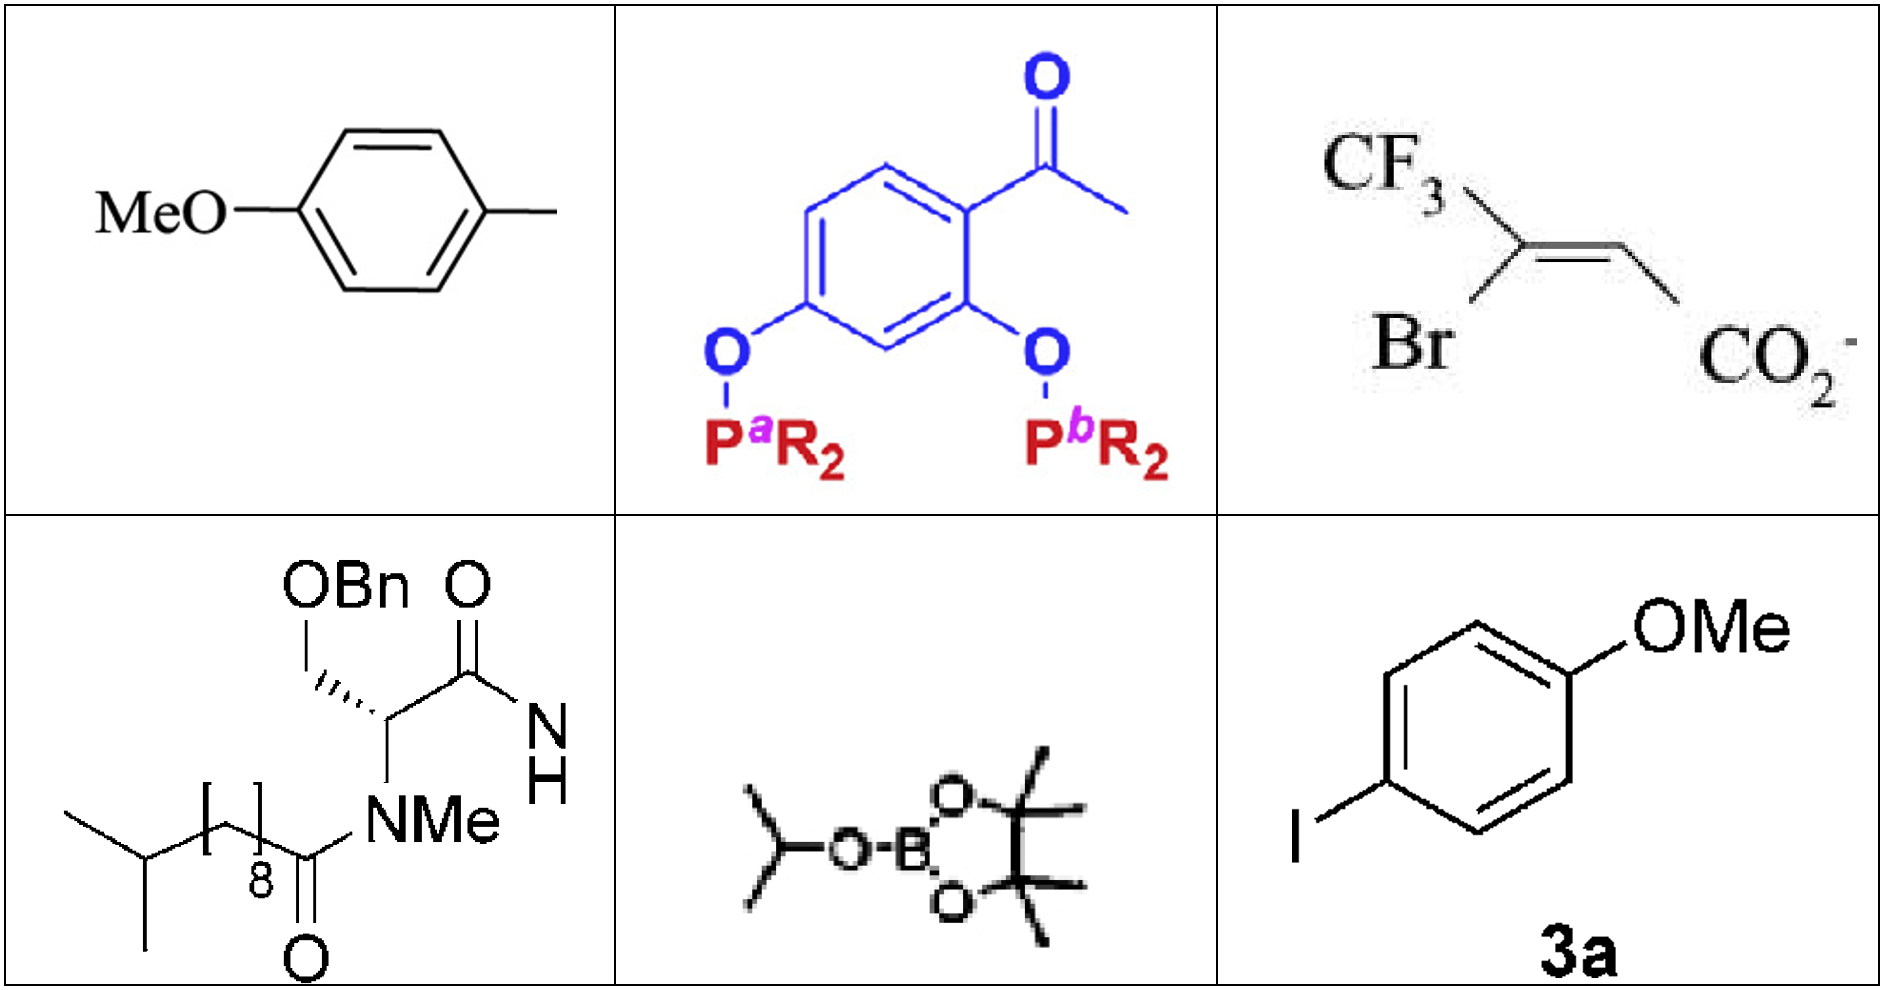
\includegraphics[scale=0.3]{imagenes/positive_examples.png}}  
%     \caption{Ejemplos de muestras positivas del dataset} 
% \end{figure}

% Los ejemplos negativos son, en cambio, imágenes que contienen rectas, curvas y otras figuras que se parecen a las formas que adquiere una molécula, pero no lo son. En esta categoría hay más imágenes, 800 en total.

% \begin{figure}[H]
% \centering
%     \fbox{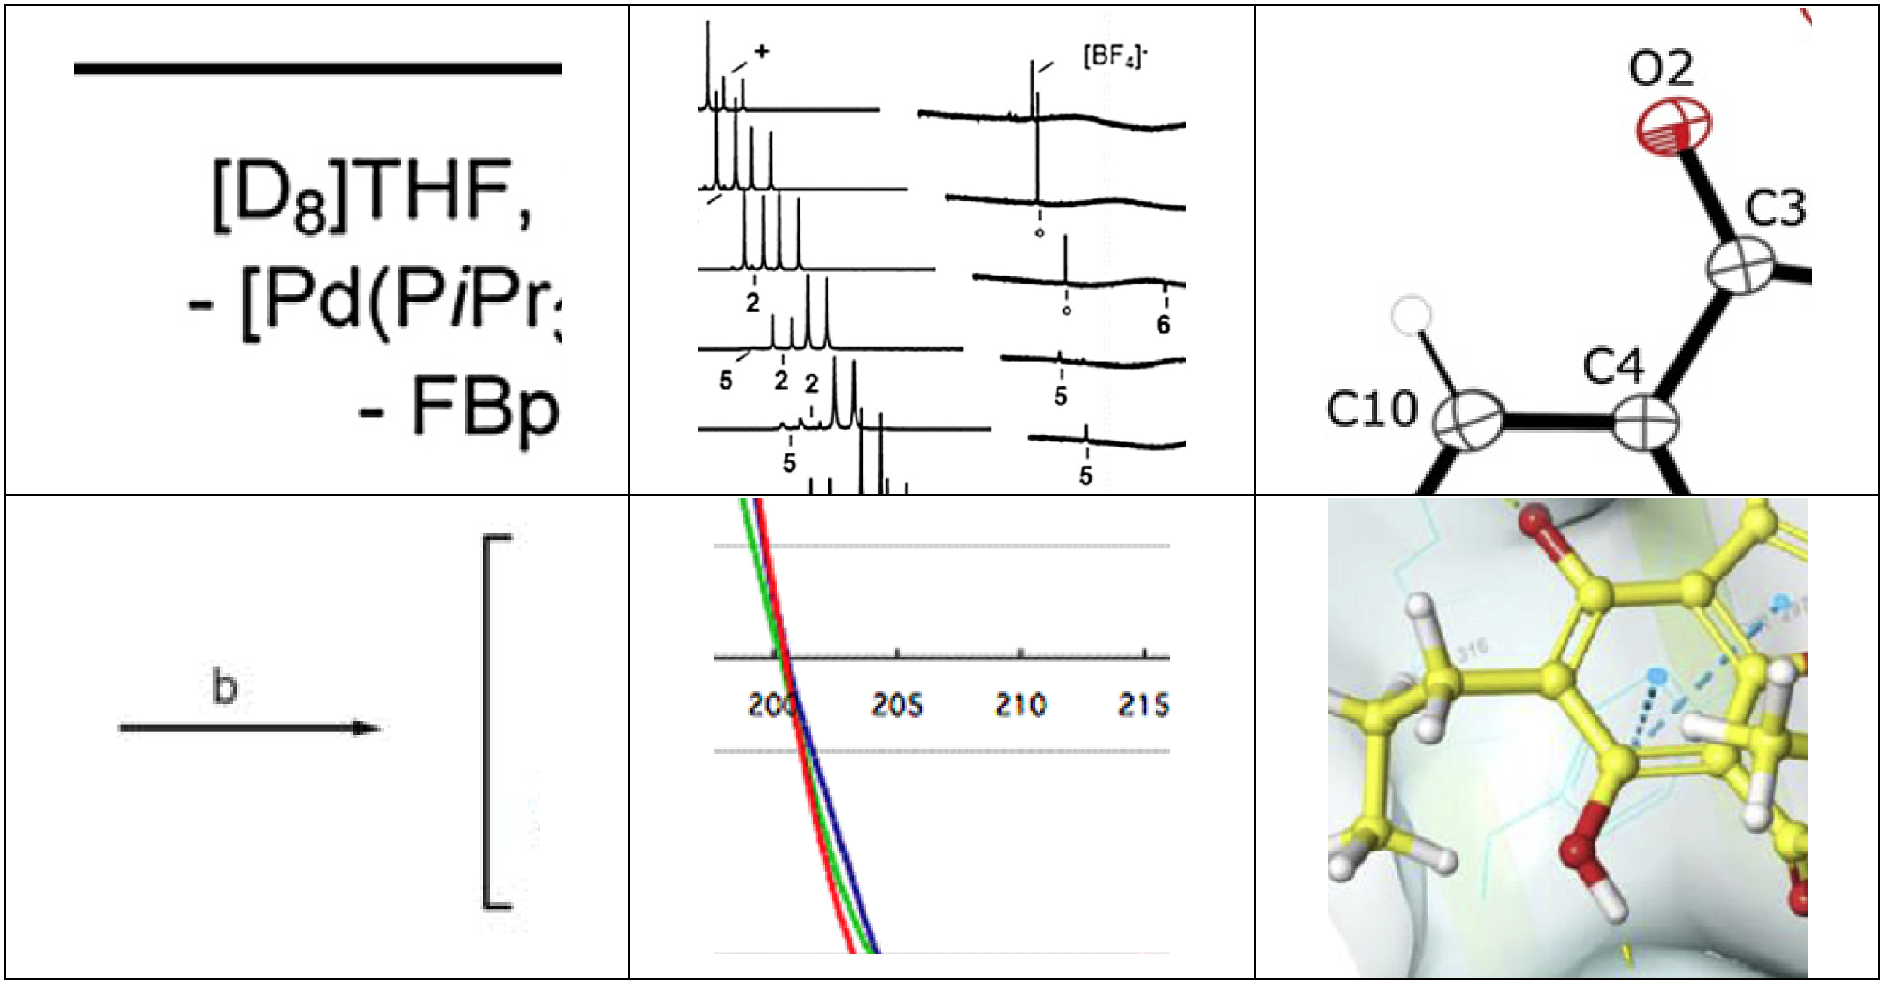
\includegraphics[scale=0.3]{imagenes/negative_examples.png}}  
%     \caption{Ejemplos de muestras negativas del dataset} 
% \end{figure}

% Estas imágenes necesitan un preprocesamiento, es necesario elegir el formato con el que se va a trabajar y dimensionarlas para que todas tengan el mismo tamaño. Debido a que el canal alfa del formato .png no se está aprovechando, decidimos convertirlas a formato .jpg y así trabajar con tres canales en nuestros modelos. Además, el modelo generativo que utilizamos está diseñado para trabajar con imágenes con este número de canales, así que será lo más adecuado.

% Lo más conveniente sería dimensionar todas las imágenes al tamaño de la más grande, así no se perdería información. Pero esto puede suponer un problema, ya que existen algunas que superan los 700x700 píxeles, y cuanto mayor es su resolución más parámetros necesitan almacenar los modelos, dando lugar a altos tiempos de ejecución, y sobre todo, a problemas con la memoria de la GPU. Las GPUs del clúster no tienen capacidad para almacenar modelos con tantos parámetros, por lo que decidimos reducir el tamaño de las imágenes a 256x256. 

% También mencionar el limitado número de ejemplos positivos que tenemos en comparación con negativos: estamos ante un conjunto de datos desbalanceado. En el momento de entrenar el clasificador, tendremos que conseguir que esté balanceado, ya sea reduciendo el número de ejemplos negativos utilizado o aplicando \textit{data augmentation} sobre los positivos. En este trabajo elegimos la segunda opción, ya que en Aprendizaje Automático cuantos más datos se utilizan en el entrenamiento, mejores modelos se obtienen y con mayor capacidad de generalización. 

% La técnica de \textit{data augmentation} consiste en aumentar el tamaño del conjunto de datos completándolo con imágenes alteradas de este. Existen bibliotecas en lenguajes de programación como Python que facilitan en gran medida esta tarea, ya que permiten indicar, entre una serie de transformaciones ya implementadas, cuáles queremos aplicar \cite{imgaug}. En nuestro caso vamos a crear tres \textit{data augmentation} diferentes, y comprobaremos cuál funciona mejor en los experimentos. La primera realizará transformaciones suaves, la segunda algo más fuertes y la tercera bastante disruptivas.

% \begin{algorithm}[H]
%     \caption{\textit{Data augmentation} 1: Transformaciones suaves}
% \begin{algorithmic}[1]
%     \State A\_veces(50\%, DesenfoqueGaussiano(sigma=[0, 0.5]))
%     \State Escalar(x: [80\%, 100\%], y: [80\%, 100\%])
%     \State Rotar([-25º, +25º])
%     \State Estirar([-5,5])
% \end{algorithmic}
% \end{algorithm}

% A cada imagen del conjunto de datos se le aplicarán estas cuatro transformaciones, la primera solamente con un 50\% de probabilidad. Los parámetros de cada transformación vienen dados en un rango, de forma que se elige un valor aleatorio en este.

% \begin{figure}[H]
% \centering
%     \begin{subfigure}{.35\textwidth}
%         \centering
%         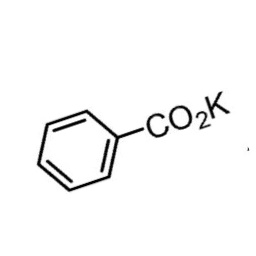
\includegraphics[width=1\linewidth]{imagenes/aug/180.jpg}
%     \end{subfigure}%
%     \begin{subfigure}{.35\textwidth}
%         \centering
%         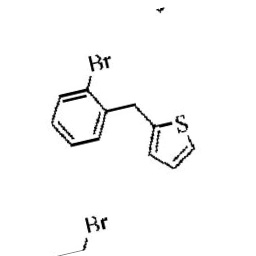
\includegraphics[width=1\linewidth]{imagenes/aug/193.jpg}
%     \end{subfigure}%

%     \bigskip

%     \begin{subfigure}{.35\textwidth}
%         \centering
%         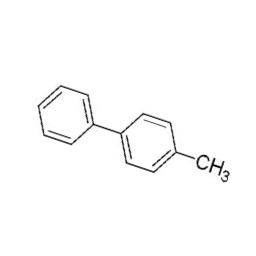
\includegraphics[width=1\linewidth]{imagenes/aug/224.jpg}
%     \end{subfigure}%
%     \begin{subfigure}{.35\textwidth}
%         \centering
%         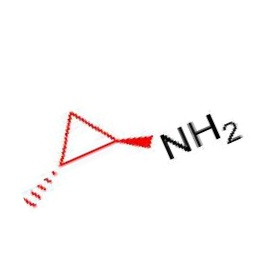
\includegraphics[width=1\linewidth]{imagenes/aug/370.jpg}
%     \end{subfigure}

%     \caption{Imágenes generadas aplicando \textit{data augmentation} 1}
% \end{figure}

% Algunos ejemplos son los que se muestran sobre este párrafo, se aprecian leves rotaciones y estiramientos de las imágenes, sin existir gran diferencia con las originales.

% \begin{algorithm}[H]
%     \caption{\textit{Data augmentation} 2: Transformaciones más fuertes}
% \begin{algorithmic}[1]
%     \State A\_veces(50\%, DesenfoqueGaussiano(sigma=[0, 0.5]))
%     \State ContrasteLineal([0.75, 1.5])
%     \State Escalar(x: [70\%, 100\%], y: [70\%, 100\%])
%     \State Rotar([-45º, +45º])
%     \State Estirar([-10,10])
%     \State Trasladar(x: [-10\%, 10\%], y: [-10\%, 10\%])
%     \State Multiplicar([0.8, 1.2], por\_canal=25\%)
%     \State RuidoGaussianoAditivo(loc=0, escala=[0.0, 0.05*255])
%     \State VoltearIzdaDcha(30\%)
% \end{algorithmic}
% \end{algorithm}

% En este caso, utilizaremos transformaciones como Multiplicar (multiplica el valor de los píxeles de la imagen por un número entre 0.8 y 1.2), RuidoGaussianoAditivo (donde a cada píxel se le añade ruido generado mediante una distribución gaussiana centrada en 0 y con desviación entre 0 y 0.05*255) o VoltearIzqdaDcha, entre otras.

% \begin{figure}[H]
% \centering
%     \begin{subfigure}{.35\textwidth}
%         \centering
%         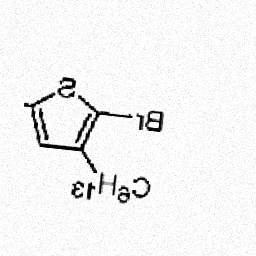
\includegraphics[width=1\linewidth]{imagenes/aug2/169.jpg}
%     \end{subfigure}%
%     \begin{subfigure}{.35\textwidth}
%         \centering
%         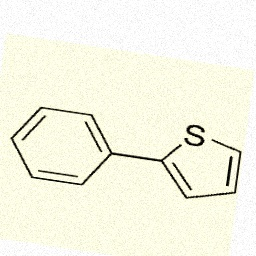
\includegraphics[width=1\linewidth]{imagenes/aug2/188.jpg}
%     \end{subfigure}%

%     \bigskip

%     \begin{subfigure}{.35\textwidth}
%         \centering
%         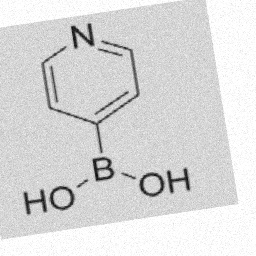
\includegraphics[width=1\linewidth]{imagenes/aug2/221.jpg}
%     \end{subfigure}%
%     \begin{subfigure}{.35\textwidth}
%         \centering
%         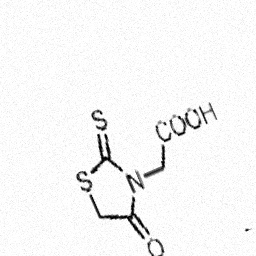
\includegraphics[width=1\linewidth]{imagenes/aug2/222.jpg}
%     \end{subfigure}

%     \caption{Imágenes generadas aplicando \textit{data augmentation} 2}
% \end{figure}

% En este caso se observan más cambios fundamentalmente debidos a las variaciones en contraste, al uso de ruido gaussiano y a la multiplicación, responsable de los cambios de color, ya que a veces se aplica a canales independientes. 

% \begin{algorithm}[H]
%     \caption{\textit{Data augmentation} 3: Transformaciones fuertes}
% \begin{algorithmic}[1]
%     \State A\_veces(50\%, DesenfoqueGaussiano(sigma=[0, 0.6]))
%     \State ContrasteLineal([0.75, 2])
%     \State Escalar(x: [70\%, 100\%], y: [70\%, 100\%])
%     \State Rotar([-45º, +45º])
%     \State Estirar([-10,10])
%     \State Trasladar(x: [-20\%, 20\%], y: [-10\%, 10\%])
%     \State Multiplicar([0.6, 1.4], por\_canal=25\%)
%     \State RuidoGaussianoAditivo(loc=0, escala=[0.0, 0.05*255], por\_canal=30\%)
%     \State VoltearIzdaDcha(20\%)
%     \State VoldearArribaAbajo(20\%)
%     \State A\_veces(70\%, TransformacionElastica(alfa=[0.75, 3], sigma=(0.2, 0.5)))
%     \State UnoEntre(Nitidez(alfa=[0, 1], lightness=[0.5, 1.5]), Emboss(alfa=[0, 1], fuerza=[0.75, 2]))
%     \State Dropout([0.01, 0.15], por\_canal=0.5)
% \end{algorithmic}
% \end{algorithm}
% % TODO: Cómo se traduce emboss al español??

% Finalmente, en esta versión de \textit{data augmentation} añadimos transformaciones que alteran en gran medida el aspecto de las imágenes. TransformacionElastica desplaza píxeles de una zona de la imagen a otra cercana, donde alfa controla la distancia con la que se produce el desplazamiento y sigma la suavidad de este, un valor bajo de sigma dará lugar a imágenes ruidosas y pixeladas. Nitidez aplica este efecto a la imagen y mezcla el resultado con la imagen original, la intensidad de la mezcla se controla con el parámetro alfa, mientras que el parámetro lightness controla el brillo de la imagen. Emboss da a la imagen un aspecto metálico, pronunciando las altas luces y sombras. Por último, Dropout da el valor 0 a cada pixel con una probabilidad entre 0.01 y 0.15. 

% \begin{figure}[H]
% \centering
%     \begin{subfigure}{.35\textwidth}
%         \centering
%         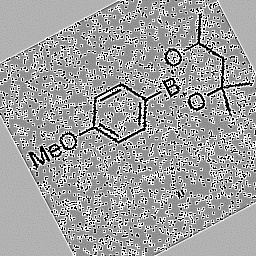
\includegraphics[width=1\linewidth]{imagenes/aug3/175.jpg}
%     \end{subfigure}%
%     \begin{subfigure}{.35\textwidth}
%         \centering
%         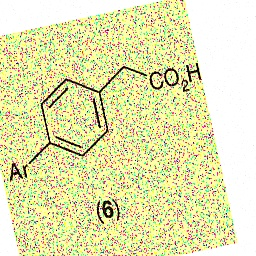
\includegraphics[width=1\linewidth]{imagenes/aug3/183.jpg}
%     \end{subfigure}%

%     \bigskip

%     \begin{subfigure}{.35\textwidth}
%         \centering
%         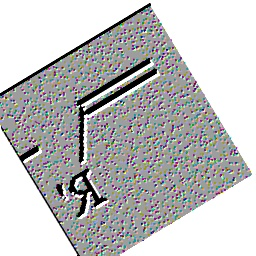
\includegraphics[width=1\linewidth]{imagenes/aug3/225.jpg}
%     \end{subfigure}%
%     \begin{subfigure}{.35\textwidth}
%         \centering
%         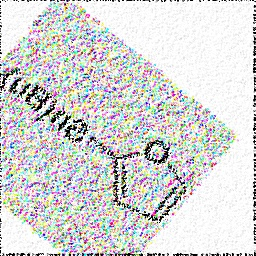
\includegraphics[width=1\linewidth]{imagenes/aug3/271.jpg}
%     \end{subfigure}

%     \caption{Imágenes generadas aplicando \textit{data augmentation} 3}
% \end{figure}

% En esta última versión las transformaciones son bastante agresivas. Se introduce mucho ruido en las imágenes y las rotaciones y los cambios en el contraste son fuertes.

% \section{Estructura del código}
% Como se menciona al principio del capítulo, la implementación se sitúa en el directorio $experiments/$, dividido en dos subdirectorios. El primero contiene el código del modelo generador de imágenes, el segundo el del clasificador: \\

% \dirtree{%
%     .1 experiments/\DTcomment{implementación del TFG}.
%     .2 taming\_transformers/\DTcomment{generador de imágenes}.
%     .3 taming-transformers/.
%     .4 configs/.
%     .4 logs/.
%     .4 train\_ngpu.sh.
%     .3 data\_generation\_and\_aug.ipynb.
%     .3 sample\_and\_clean\_molecules.ipynb.
%     .3 sampling\_experiment.ipynb.
%     .3 functions.py.
%     .2 image\_classifier/\DTcomment{clasificador de imágenes}.
%     .3 saved\_models/.
%     .3 datasets.py.
%     .3 functions.py.
%     .3 grid\_search.py.
%     .3 models.py.
%     .3 train.py.
%     .3 train\_ngpu.sh.
% }

% \subsection{Generador de imágenes sintéticas}
% Uno de los objetivos del proyecto es construir un modelo que nos permita generar imágenes sintéticas de moléculas. 

% \section{Ejecución y reproducibilidad}
% Como ejecutar los scripts y semillas utilizadas